\begin{figure}[!h]
	\begin{center}
		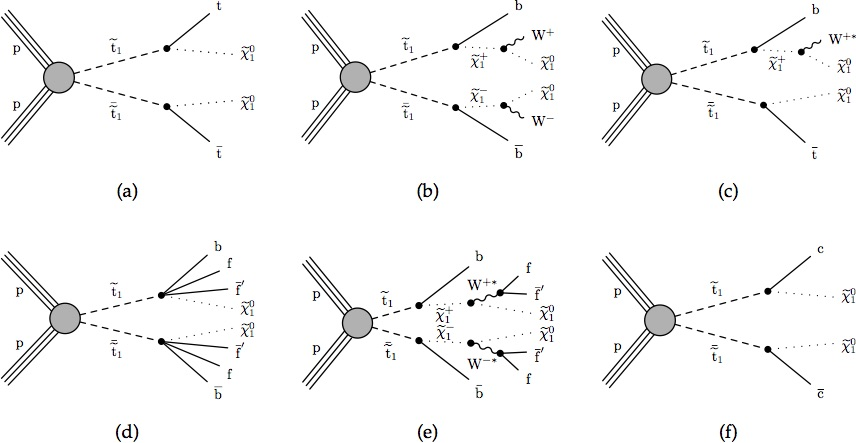
\includegraphics[width=1.00\textwidth]{T2tt_all.jpg}
	\end{center}
	\caption[Direct Top Squark Production]{Feynman diagrams for the direct \st{} production in SUSY. The allowed decay modes are (a) T2tt, (b) T2bW, (c) T2tb, (d, e) T2fbd, and (f) T2cc. }
	\label{fig:stop-direct-production}
\end{figure}

\begin{figure}[!h]
	\begin{center}
		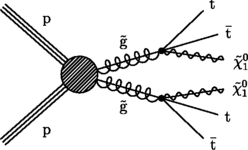
\includegraphics[width=0.32\textwidth]{T1tttt.png}
		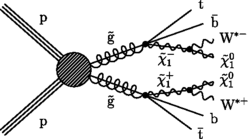
\includegraphics[width=0.32\textwidth]{T1ttbb.png} \\
		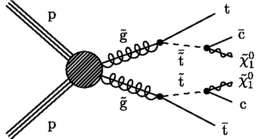
\includegraphics[width=0.32\textwidth]{T5ttcc.png}
		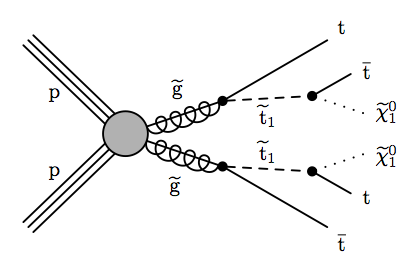
\includegraphics[width=0.32\textwidth]{T5tttt.png} \\
	\end{center}
	\caption[Gluino Mediated Top Squark Production]{Feynman diagrams for the indirect \st{} production in SUSY. The allowed decay modes are T1tttt (top left), T1ttbb (top right), T5ttcc (bottom left), and T5tttt (bottom right).
	}
	\label{fig:stop-gluino-production}
\end{figure}
